\chapter{Introduction to Radiation Physics}

\section{Measuring Radiation}

One quantitative measure that astronomers use when observing a light source is the amount of radiation received. Quantifying this amount involves several related but distinct concepts. We discuss these measures below.

\subsection{Total Energy Emitted}

A source's total light output can be described by the total amount of energy emitted over its lifetime, at all frequencies, and in all directions. However, this comprehensive measure is impractical for direct observation since we can only measure radiation over finite time periods. Instead, we focus on measurements normalized by time.

\subsection{Luminosity}

Luminosity (L) or power is the rate at which energy is emitted by a source, expressed in watts (W) or ergs per second (erg s\textsuperscript{-1}). It is calculated by dividing the total emitted energy by the time period over which it was emitted.

\subsection{Flux}

Flux (F) measures the amount of light energy per unit time per unit area that we detect from a source. It is normalized by dividing the detected power by the effective area of the telescope receiving the radiation. Flux is expressed in units of joules per second per square meter (J s\textsuperscript{-1} m\textsuperscript{-2}) or watts per square meter (W m\textsuperscript{-2}). \\

The relationship between flux and luminosity for an isotropic source at distance \( d \) is given by:
\[ F = \frac{L}{4 \pi d^2} \]

\subsection{Flux Density}

Flux density ($F_{\nu}$ or $F_{\lambda}$) refers to the flux per unit frequency or wavelength range observed. It is calculated by dividing the detected flux by the frequency or wavelength bandwidth (\( \Delta \nu \) or \( \Delta \lambda \)). Flux density is crucial in characterizing the spectral properties of sources. \\

For radio astronomy, flux density per unit frequency (\( S_{\nu} \)) in janskys (Jy) is a commonly used unit:
\[ 1 \text{ Jy} = 10^{-26} \text{ W m}^{-2} \text{ Hz}^{-1} \]

\subsection{Intensity}

Intensity $I_{\nu}$ or $I_{\lambda}$, also known as specific intensity or surface brightness, is the flux density per unit solid angle. It measures the amount of energy radiated per second per unit area per unit solid angle of the source. Intensity is independent of distance and provides insights into the microscopic radiation processes of the emitting object. \\

The relationship between flux density and intensity is:
\[ I_\nu = \frac{F_\nu}{\Omega} \]

where \( \Omega \) is the solid angle subtended by the source. Intensity is commonly expressed in units of watts per square meter per hertz (W Hz\textsuperscript{-1} m\textsuperscript{-2} sr\textsuperscript{-1}) or watts per square meter per nanometer (W nm\textsuperscript{-1} Hz\textsuperscript{-1} m\textsuperscript{-2} sr\textsuperscript{-1}) depending on the wavelength regime.

\subsection{Relation between Intensity and Electric Field}

Intensity is related to the electric field strength of the radiation waves via the Poynting vector. The intensity of radiation is proportional to the square of the electric field amplitude \( E_0 \).

\[ I_\nu \propto E_0^2 \]

This relationship underscores the fundamental connection between the electromagnetic wave properties and the measurable quantities of radiation intensity. \\

In summary, astronomers employ various measures such as luminosity, flux, flux density, and intensity to quantitatively describe the amount of radiation emitted by astronomical sources. Each measure provides unique insights into the nature and properties of celestial objects across different wavelength regimes.

\section{Blackbody Radiation}
\label{sec:blackbodyradiation}

At the start of the twentieth century, Max Planck's discovery that light's energy is quantized into packets called photons was pivotal. Blackbody radiation, the light emitted by a body that absorbs all incident light, is a key concept. This radiation helps us understand how hot objects cool by emitting light. \\

A blackbody is an idealized object that emits radiation solely based on its temperature, with no reflection or transmission. The interactions between photons and particles within the blackbody result in a thermal equilibrium, where both have the same temperature. \\

Photons are described by Bose–Einstein statistics, which help in determining the distribution of photon energies in thermal equilibrium. The energy distribution function of photons is directly related to the spectrum of emitted light, known as the Planck function:

\begin{equation}
	B_\nu (T) = \frac{2h\nu^3}{c^2} \frac{1}{e^{h\nu/kT} - 1}
	\label{eq:planckfunctionfrequency}
\end{equation}


where:
\begin{itemize}
    \item \(h = 6.626 \times 10^{-34} \, \text{J s} = 6.626 \times 10^{-27} \, \text{erg s}\) is Planck’s constant
    \item \(k = 1.38 \times 10^{-23} \, \text{J K}^{-1} = 1.38 \times 10^{-16} \, \text{erg K}^{-1}\) is Boltzmann’s constant
    \item \(c\) is the speed of light
    \item \(\nu\) is the frequency of the observation
    \item \(T\) is the temperature of the radiating body in Kelvins
\end{itemize}

In the Planck function given in Equation~\eqref{eq:planckfunctionfrequency}, written as $B_\nu(T)$, the subscript $\nu$ indicates that the spectral measure is per unit frequency and $B$ represents the intensity, or brightness, of the blackbody radiation and has units of intensity, \( \text{W m}^{-2} \text{Hz}^{-1} \text{sr}^{-1} \). Since this is an intensity, the Planck function can also be expressed as flux per unit wavelength per steradian, which is denoted as $B_\lambda(T)$. Radio astronomers generally express the Planck function using $B_\nu(T)$. The equation for $B_\lambda(T)$ is

\begin{equation}
	B_\lambda (T) = \frac{2hc^2}{\lambda^5} \frac{1}{e^{hc / \lambda k T} - 1}
	\label{eq:planckfunctionwavelength}
\end{equation}


It is very important to understand and appreciate that, even though \(B_\nu\) and \(B_\lambda\) represent the same concept, they are not the same numerical quantity or even the same function. We discuss in more detail about the difference between these functions later in this section. We first discuss some important features of the Planck function. \\

Figures~\ref{fig:planckfunctionnu} and~\ref{fig:planckfunctionlambda} display the log-log plots of these functions. Blackbody emission is a continuous spectrum that reaches zero at \(\nu = 0\) (owing to the \(\nu^3\) term), increases to some peak value as \(\nu\) increases, and then decreases and reaches zero again at \(\nu = \infty\) (owing to the exponential term). Note that the Planck function depends only on the body’s temperature and the frequency of the radiation. No other characteristic of the body is relevant. In other words, the intensity of radiation that a blackbody emits at any given frequency depends only on its temperature. \\

\begin{figure}[H]
	\centering
	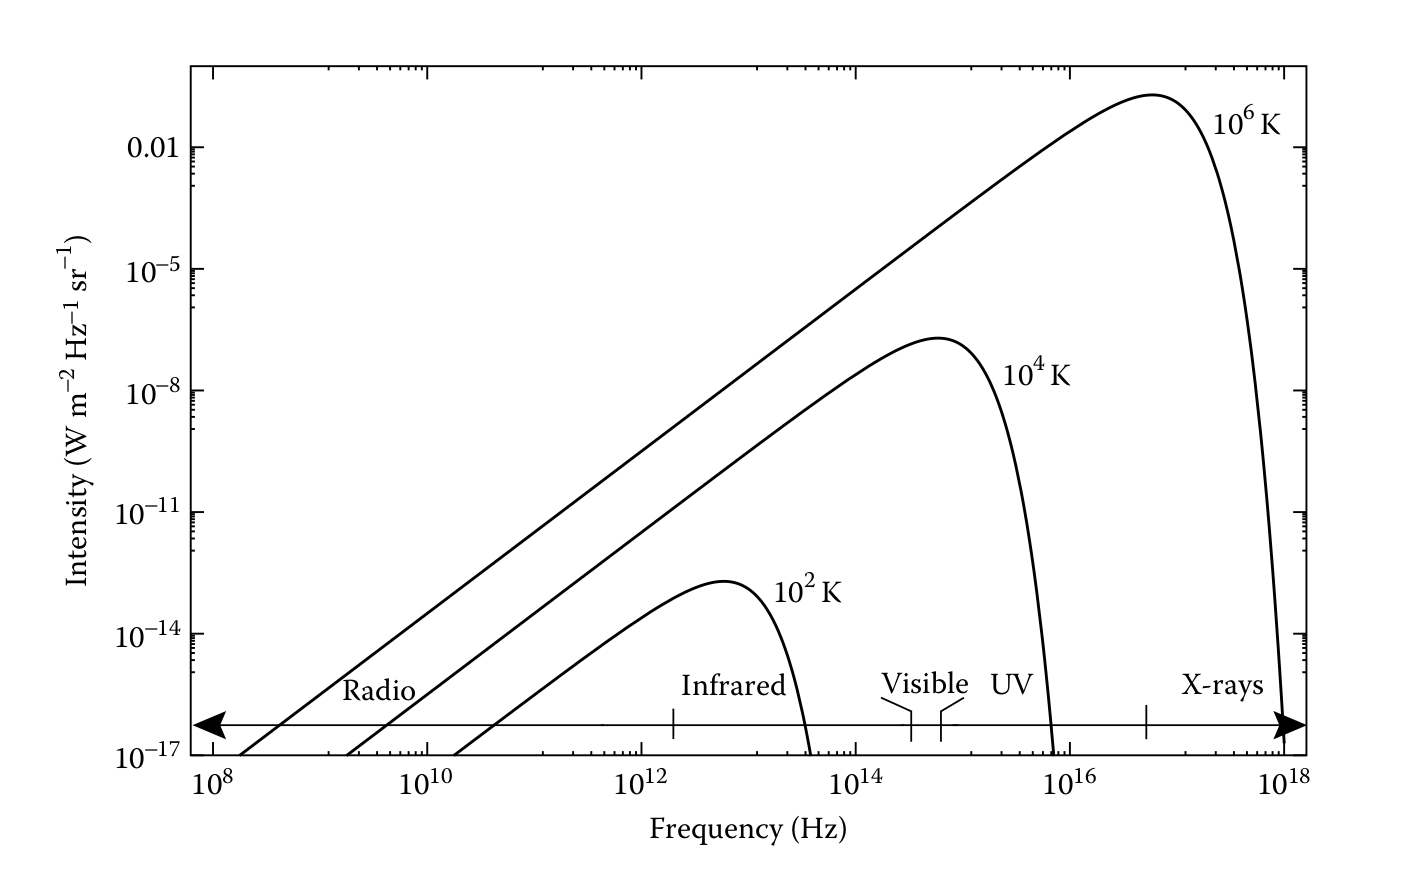
\includegraphics[width=0.7\textwidth]{Images/B_nu_plot.png}
	\caption{Log-log plot of $B_{\nu}(T)$ versus $\nu$ for three different temperatures.}
	\label{fig:planckfunctionnu}
\end{figure}

\begin{figure}[H]
	\centering
	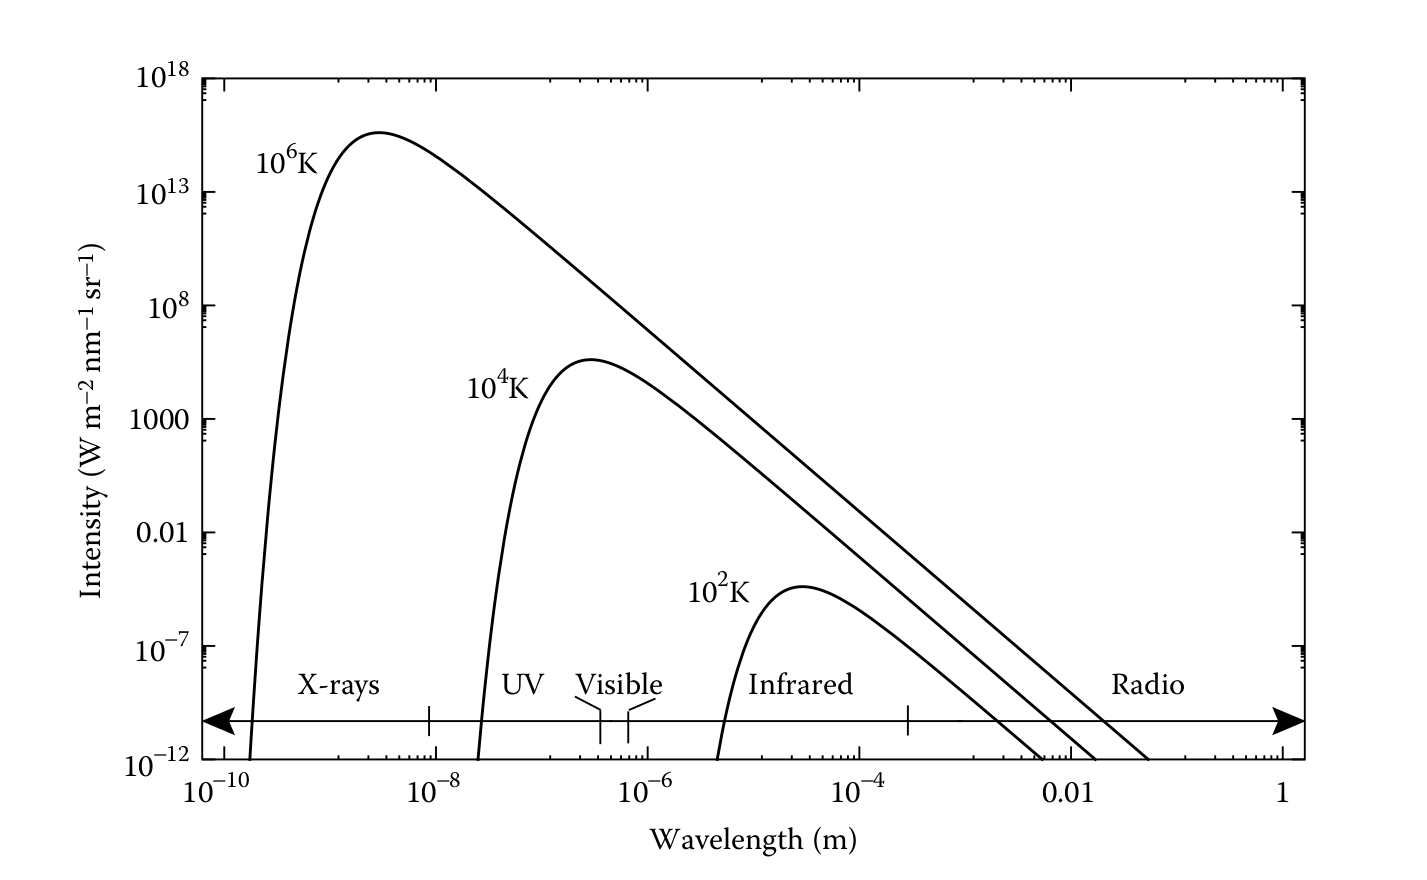
\includegraphics[width=0.7\textwidth]{Images/B_lambda_plot.png}
	\caption{Log-log plot of $B_{\lambda}(T)$ versus $\lambda$ for three different temperatures.}
	\label{fig:planckfunctionlambda}
\end{figure}

The total flux of radiation (\(\text{W m}^{-2}\)) emitted by the body can be obtained by integration of the Planck function over frequency and solid angle. The result shows that the total flux is given by

\begin{equation}
	F = \sigma T^4
	\label{eq:stefanboltzmannlaw}
\end{equation}

where \(\sigma\) is the Stefan-Boltzmann constant. This is an expression of the Stefan–Boltzmann law. Another very useful result can be obtained by finding the frequency of the peak intensity of the Planck function. This frequency, \(\nu_\text{max}\), is proportional to the body’s temperature and is given by Wien’s displacement law, which states

\[
\nu_\text{max} = 2.82 \frac{kT}{h}
\]

Finally, it is also useful to calculate the brightness temperature of a source whose intensity is \(I_\nu\). This brightness temperature, \(T_B\), is the temperature at which a blackbody would emit with an intensity equal to \(I_\nu\). That is, it is found by solving for \(T\) in the expression

\[
I_\nu = B_\nu(T)
\]

As mentioned above, radio astronomers typically express the Planck function using frequency (\(\nu\)) rather than wavelength (\(\lambda\)). Radio astronomers also express the Planck function in a modified form using temperature units. The brightness temperature of a source whose specific intensity is \(I_\nu\) is defined as the temperature of a blackbody that would emit the same specific intensity, \(T_B\), at the frequency \(\nu\). The Planck function in the Rayleigh–Jeans approximation can be expressed as

\[
B_\nu(T) \approx \frac{2\nu^2 kT}{c^2}
\]

The brightness temperature of a source with intensity \(I_\nu\) is then

\[
T_B \approx \frac{I_\nu c^2}{2k\nu^2}
\]

\section{Rayleigh-Jeans Approximation}

At most radio wavelengths, the Planck function can be approximated by a much simpler expression, which makes for much easier math when using it. At most radio wavelengths, the frequency, $\nu$, is so small that $\frac{h \nu}{k T} \ll 1$ for any reasonable temperature. The exponential in the denominator of the Planck function then can be approximated by a Taylor series expansion, yielding

\begin{equation}
\frac{1}{e^{h\nu/kT} - 1} \approx \frac{kT}{h\nu} \quad \text{for} \quad \frac{h\nu}{kT} \ll 1
\label{eq:taylor}
\end{equation}

and so,

\begin{equation}
B_\nu (T) \approx \frac{2h\nu^3}{c^2} \cdot \frac{kT}{h\nu} = \frac{2k\nu^2}{c^2} T
\label{eq:rayleigh_jeans_freq}
\end{equation}

or

\begin{equation}
B_\nu (T) \approx \frac{2kT}{\lambda^2}
\label{eq:rayleigh_jeans_wave}
\end{equation}

Note how simple this expression is in comparison to the Planck function (Equation~\eqref{eq:planckfunctionfrequency}). This expression is very useful, provided you are in the realm where $\frac{h \nu}{k T} \ll 1$. This expression is known as the Rayleigh--Jeans approximation, often referred to as the Rayleigh--Jeans law.

\clearpage

\section{Brightness Temperature}

Brightness temperature (\( T_B \)) is an important parameter in radio astronomy, providing a convenient way to describe the intensity of radiation using the Rayleigh–Jeans approximation. This approximation shows that at radio wavelengths, the intensity (\( B_\nu(T) \)) of radiation emitted by a blackbody is directly proportional to its temperature (\( T \)), i.e., \( B_\nu(T) \propto T \). \\

At radio wavelengths, intensity and temperature of blackbody sources can be used interchangeably and are linearly related by \( \frac{2k}{\lambda^2} \). In the Rayleigh–Jeans approximation, the brightness temperature is defined as:

\[
T_B = \frac{\lambda^2}{2k} I_\nu
\]

\( T_B \) is a property of the radiation, not the emitting object. For an opaque thermal source, \( T_B \) directly represents the object's temperature. However, it only equals the source's temperature when the source is both thermal and opaque. \\

At higher frequencies or lower temperatures, where \( h\nu \) is not much smaller than \( kT \), the Rayleigh–Jeans approximation is insufficient. In such cases, the full Planck function must be used:

\[
I_\nu = B_\nu(T_B) = \frac{2h\nu^3}{c^2} \left( \frac{1}{e^{h\nu/kT_B} - 1} \right)
\]

Brightness temperature measures intensity and equals the temperature of an opaque thermal source at low frequencies. For non-thermal radiation (e.g., synchrotron radiation), \( T_B \) is not related to the source temperature but still describes radiation intensity. \\

Temperature descriptions for intensity or radiation power also appear in other contexts, such as antenna temperature, noise temperature, receiver temperature, and system temperature, representing power per unit frequency in radio telescope observations. \\

\clearpage

\section{Coherent Radiation}

The radio-wavelength radiation emitted by an individual electron is undetectable by any radio telescope; what we detect is the sum of emissions from many electrons. There are two main ways electromagnetic waves from different electrons can combine, which significantly affects how we treat the radiation mathematically and its physical properties. \\

Imagine a single electron oscillating at a fixed frequency, emitting electromagnetic waves at a single wavelength. If multiple wave chains, all in phase, join this initial chain, they amplify the initial wave constructively, resulting in coherent radiation. This is similar to what happens in a laser. \\

In contrast, incoherent radiation occurs when many unrelated electrons emit radiation independently, as in an incandescent light bulb. The resulting waves have random phases and cannot be modeled by a single chain of sine waves.

\begin{figure}[H]
	\centering
	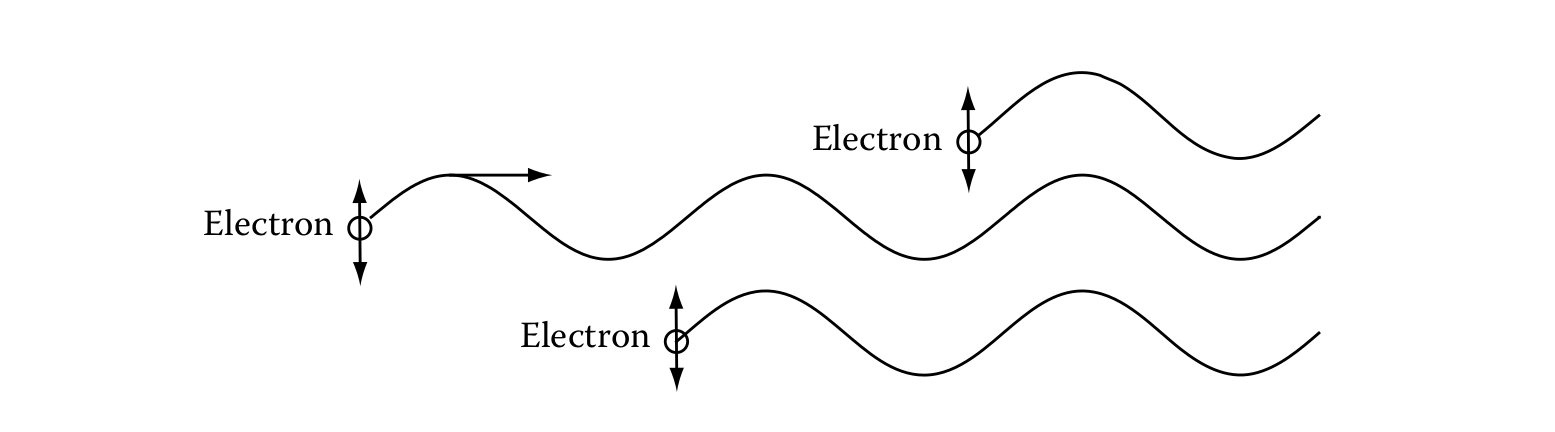
\includegraphics[width=0.5\textwidth]{Images/coherent_radiation.png}
	\caption{Creation of Coherent Radiation.}
	\label{fig:coherent_radiation}
\end{figure}

Mathematically, coherence of radiation means that at any location in space and time, the radiation has a specific phase. To understand coherence, consider two electromagnetic wave chains with identical frequencies and directions, but with a phase difference. Representing the waves as cosines:

\[
E_1 = E_0 \cos(\omega t)
\]
\[
E_2 = E_0 \cos(\omega t + \Delta \phi)
\]

Their sum is:

\[
E_1 + E_2 = E_0 \cos(\omega t) + E_0 \cos(\omega t + \Delta \phi)
\]

The intensity (\( I \)) is proportional to the square of the electric field, averaged over time. The intensity of each wave chain is:

\[
I_1 = I_2 = \alpha E_0^2 / 2
\]

The total intensity is:

\[
I_{\text{total}} = \alpha (E_1 + E_2)^2 = \alpha E_0^2 \left[1 + \cos(\Delta \phi)\right]
\]

When waves are in phase (\( \Delta \phi = 0 \)), \( \cos(\Delta \phi) = 1 \), and the total intensity is four times that of an individual wave. For incoherent light, the interference term averages to zero, resulting in the total intensity being the sum of individual intensities. \\

In summary, incoherent light results in a total intensity equal to the sum of component intensities, while coherent light's intensity grows as the square of the sum of the component intensities. Despite the differing intensities, the total energies remain conserved, with coherent light having a higher intensity over a smaller wavelength range and a narrower beam.


\clearpage

\section{Interference of Light}

Interference of light is crucial for understanding the functioning of radio telescopes. This concept was famously demonstrated by Thomas Young's double-slit experiment, which established the wave nature of light in the early nineteenth century. \\

The classroom demonstration typically uses a laser beam, which is highly coherent, shining on a double slit. The light from the slits combines to form an interference pattern on a screen. The pattern arises because the path lengths from the two slits to the screen differ, causing phase differences. At the midpoint between the slits, the path lengths are equal, so the phases are the same, resulting in constructive interference and a bright spot. At points offset from the midpoint, the path difference causes destructive interference, creating dark regions or nulls. \\

A schematic of Young's double-slit experiment and the resulting interference patterns is shown in Figure~\ref{fig:double_slit}. Despite using sunlight, which is not coherent, Young observed interference patterns because he passed the sunlight through a pinhole before the slits, enhancing spatial coherence. 

\begin{figure}[H]
    \centering
    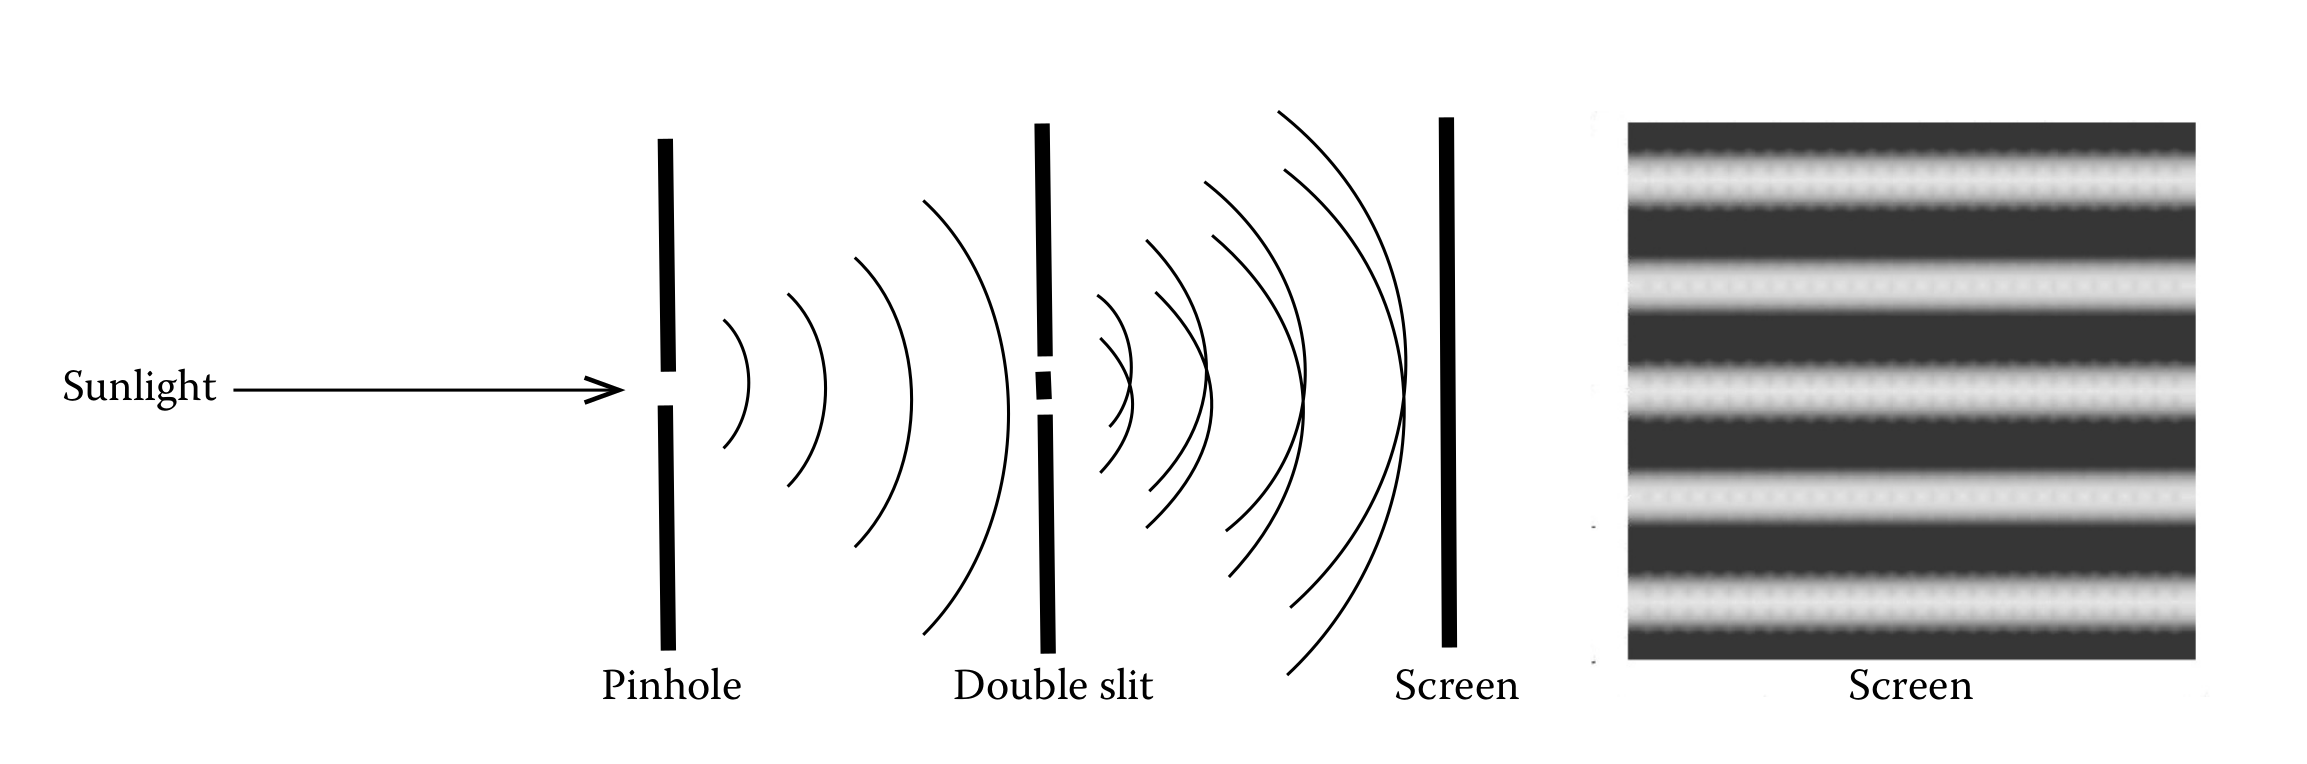
\includegraphics[width=0.8\textwidth]{Images/double_slit.png} 
    \caption{Schematic representation of Young’s double-slit experiment is shown on the left and the display of the bright and dark lines that appear on the screen due to interference is shown on the right.}
    \label{fig:double_slit}
\end{figure}

Interference patterns do not require all wave chains to be in phase. Each wave chain passing through the slits produces its own interference pattern. The total intensity pattern is the sum of these individual patterns. However, a range of frequencies or directions degrades the pattern, leading to partial coherence. Laser beams exhibit high spatial and temporal coherence, but no source is perfectly coherent. \\

Young used a pinhole to create wave fronts from a single point, ensuring high spatial coherence. Despite sunlight being blackbody radiation with all wavelengths, the human eye's limited wavelength sensitivity allowed Young to see the interference pattern, effectively filtering the light by wavelength. \\

Using coherent light sources in double-slit demonstrations simplifies observing well-defined nulls and peaks. However, understanding that partial coherence can still produce interference patterns is essential in radio astronomy. Observations involve a range of wavelengths and sources with finite spatial coherence, and the phases of the radiation are usually random. This understanding is crucial for appreciating the resolution limits of radio telescopes and the technique of interferometry or aperture synthesis.

\clearpage

\section{Polarization of Light}

The direction of the electric field in an electromagnetic wave is described by its polarization. For waves traveling along the \(+z\)-axis, the electric field (\(\vec{E}\)) oscillates perpendicular to the direction of travel, typically in the \(xy\)-plane, with the magnetic field (\(\vec{B}\)) perpendicular to both \(\vec{E}\) and the direction of travel.

\begin{figure}[H]
    \centering
    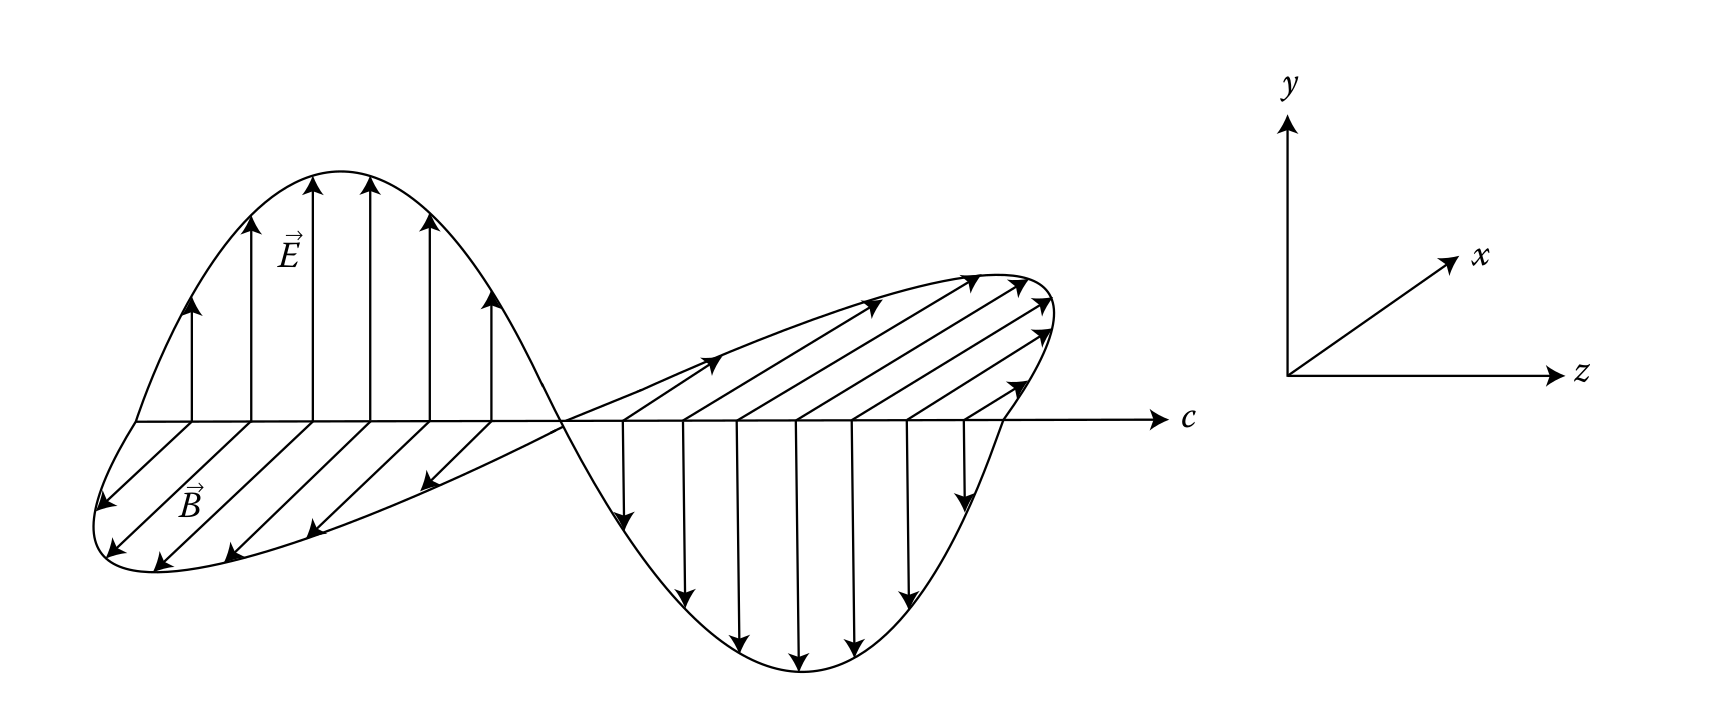
\includegraphics[width=0.4\textwidth]{Images/polarization_wave.png}
    \caption{Propagation of plane electromagnetic waves along the z-axis with the electric field oscillating along the y-axis.}
    \label{fig:polarization_wave}
\end{figure}

The electric field can oscillate in any direction within the \(xy\)-plane, affecting electrons differently based on their movement constraints. An electron constrained to move vertically will only be accelerated by vertically polarized waves.

\begin{figure}[H]
    \centering
    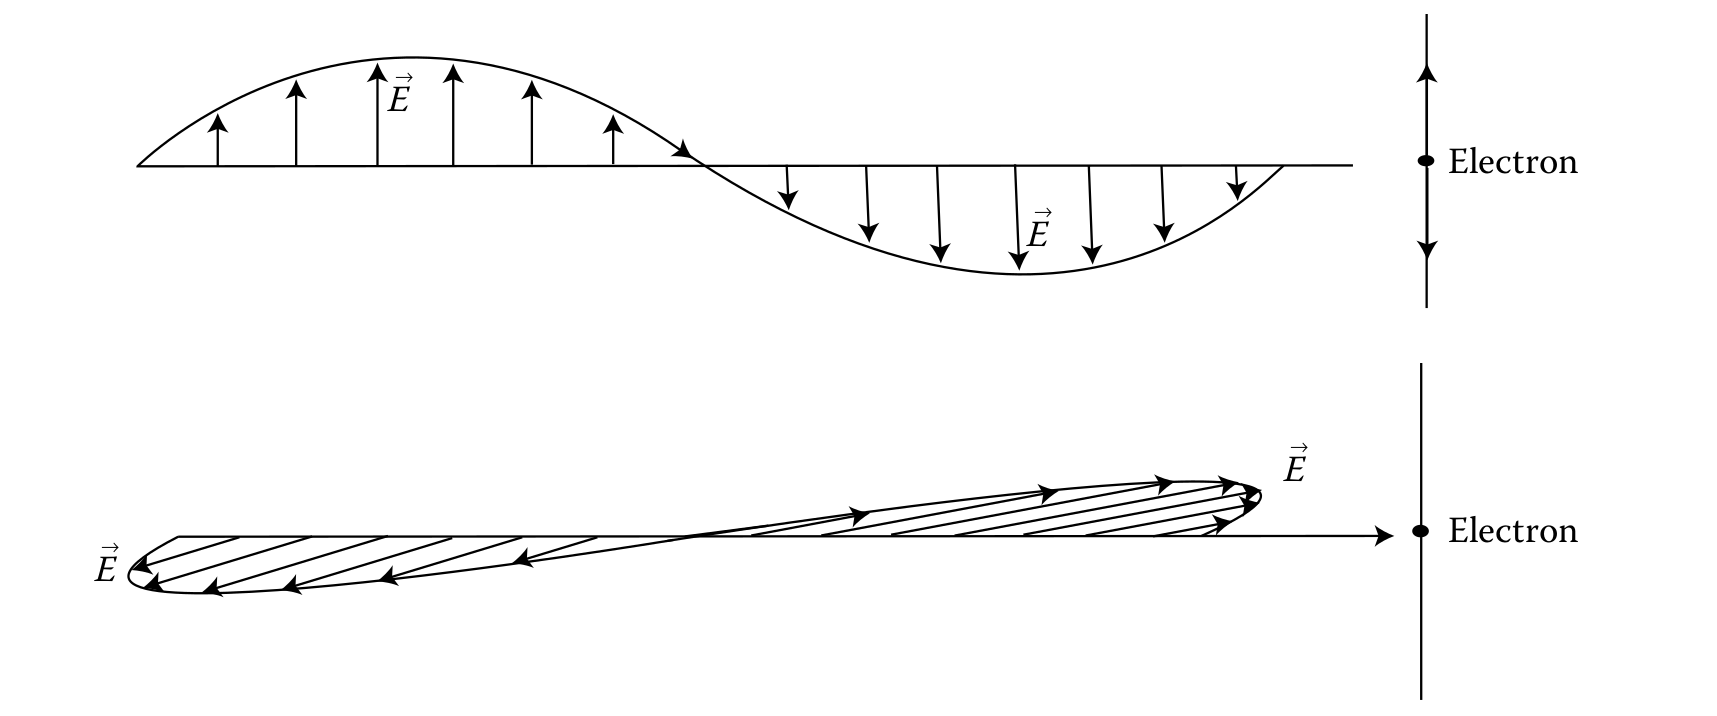
\includegraphics[width=0.4\textwidth]{Images/polarization_electron.png}
    \caption{An electron moving vertically is accelerated by vertically polarized waves but unaffected by horizontally polarized waves.}
    \label{fig:polarization_electron}
\end{figure}

Any electric field vector can be described by its components along the \(x\)- and \(y\)-axes (horizontal and vertical polarization).

\begin{figure}[H]
    \centering
    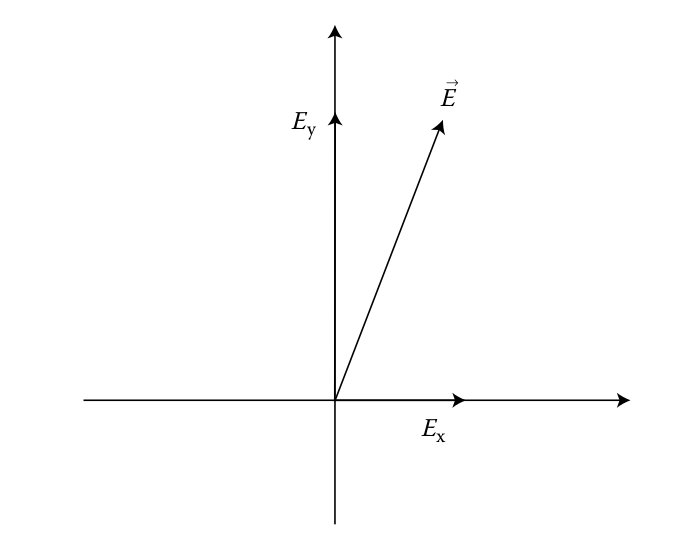
\includegraphics[width=0.25\textwidth]{Images/polarization_components.png}
    \caption{Total electric field vector described by its x- and y-components.}
    \label{fig:polarization_components}
\end{figure}

When the \(x\)- and \(y\)-components are out of phase, the total electric field vector rotates, leading to different polarization types:
\begin{enumerate}
	\item \textbf{Linear polarization}: \(\vec{E}\) oscillates in a fixed direction.
	\item \textbf{Circular polarization}: \(\vec{E}\) rotates with constant magnitude, describing a circle.
	\item \textbf{Elliptical polarization}: \(\vec{E}\) describes an ellipse.
\end{enumerate}

\clearpage

\section{Cosmic Microwave Background}

The Cosmic Microwave Background (CMB) is the thermal radiation left over from the Big Bang. It is a faint glow of light that fills the universe in all directions. The CMB is a critical piece of evidence supporting the Big Bang theory and provides a wealth of information about the universe's early history. \\

The CMB was first discovered by Arno Penzias and Robert Wilson in 1965. They were conducting radio astronomy experiments using a horn antenna at Bell Labs in New Jersey when they detected an unexpected background noise. After ruling out all possible sources of interference, they realized they had discovered the CMB. \\

We use data from COBE~\cite{1990ApJ...354L..37M} Satellite to fit the Planck function to the CMB data. We fit the Planck function to the data and determine the temperature of the CMB. The Planck function is already defined in section~\ref{sec:blackbodyradiation}.

\begin{figure}[H]
	\centering
	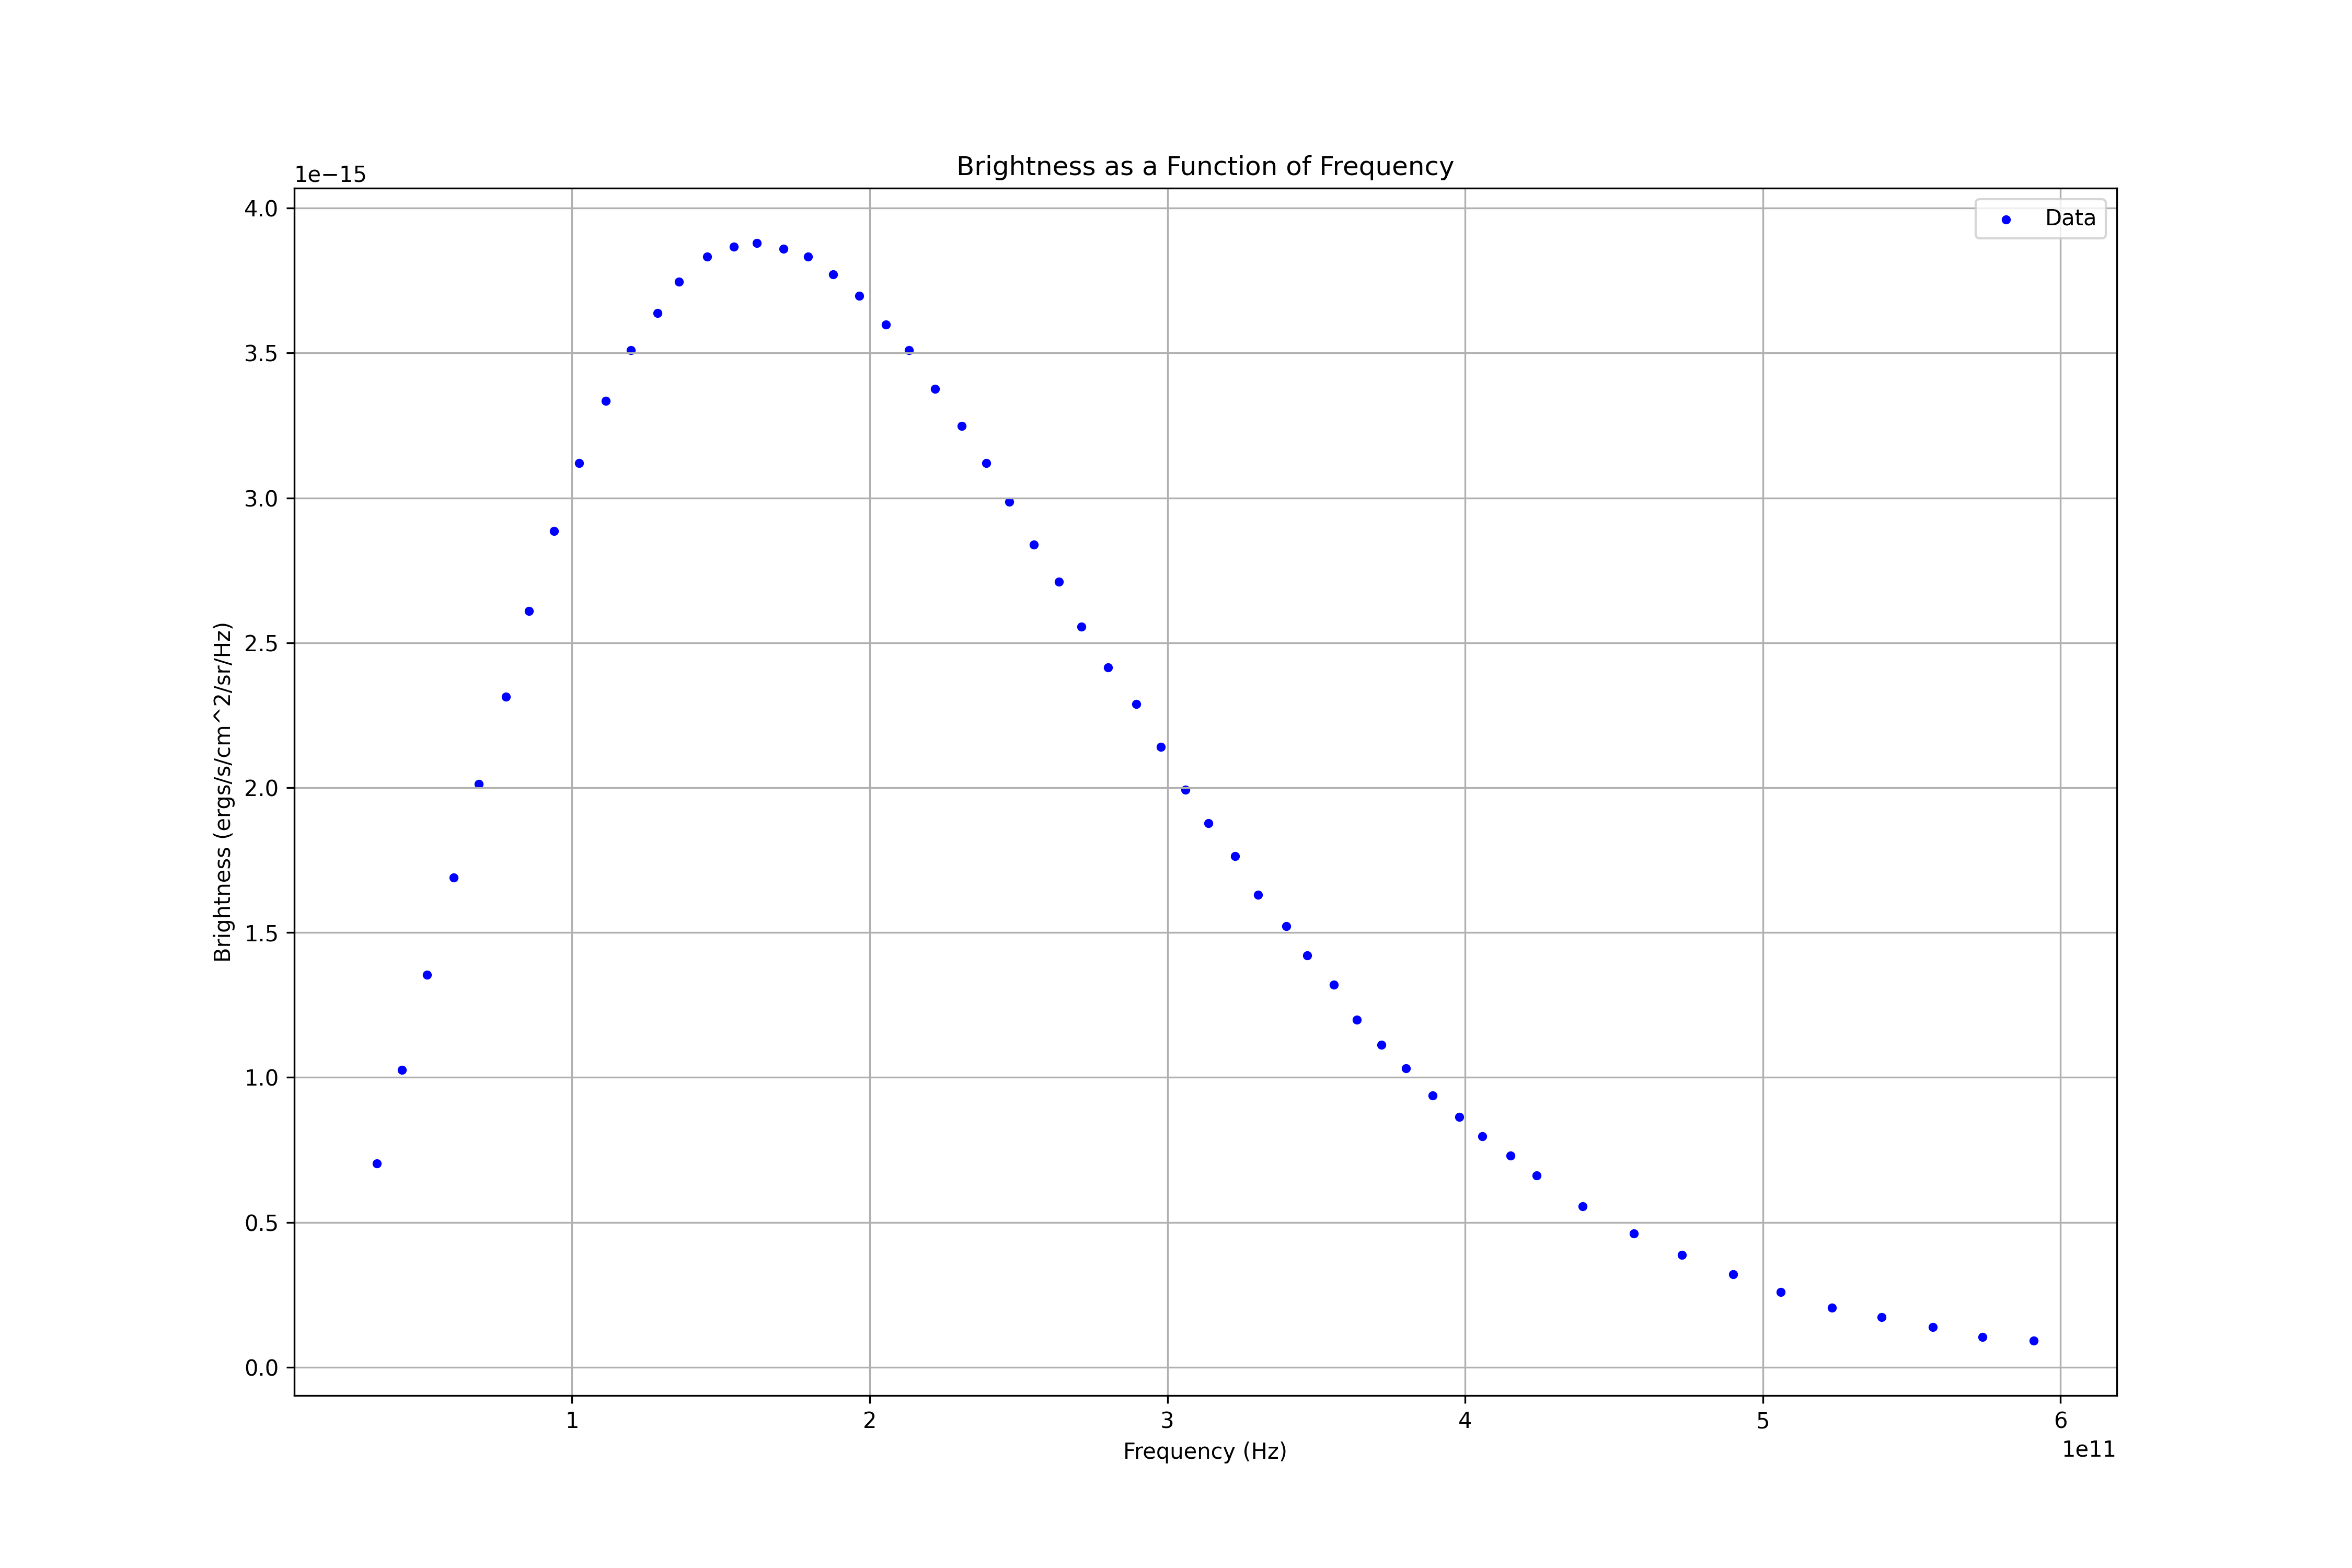
\includegraphics[width=\textwidth]{Images/COBE_CMB_data.png}
	\caption{Plotted CMB Data}
	\label{fig:cmb_fit}
\end{figure}

Using the blackbody function, we get the optimized CMB temperature to be \textbf{2.738305 K.}

\clearpage

\section{Hydrogen 21cm Line \& Galaxy Rotation Curve}

The Hydrogen $21$cm line is a very important spectral line important in radio astronomy as it is used to study the distribution of neutral atomic hydrogen in the interstellar medium. The $21$cm line is a hyperfine transition of the hydrogen atom, which occurs due to the spin-flip transition of the electron in the hydrogen atom. This line is important in studying the dynamics of galaxies and the distribution of hydrogen in the Universe. \\

The $21$cm line is used to study the rotation curve of galaxies. The rotation curve of a galaxy is a plot of the orbital velocity of the stars and gas in the galaxy as a function of the distance from the center of the galaxy. The rotation curve of a galaxy is important in studying the mass distribution of the galaxy. The rotation curve of a galaxy is used to study the dark matter distribution in the galaxy. \\

To obtain the galaxy rotation curve, we will use synthetic spectra available for different spectrums of different distance intervals within that is a Hydrogen 21 cm line at a Doppler velocity. We fit for the Doppler velocity of the 21 cm line for each distance. To do so, we fit a gaussian to the spectral line and determine the central frequency. We use the displacement from the expected value to find the velocity. Once all lines are done, plot the velocities as a function of distance from the centre of our galaxy.

\begin{figure}[H]
	\centering
	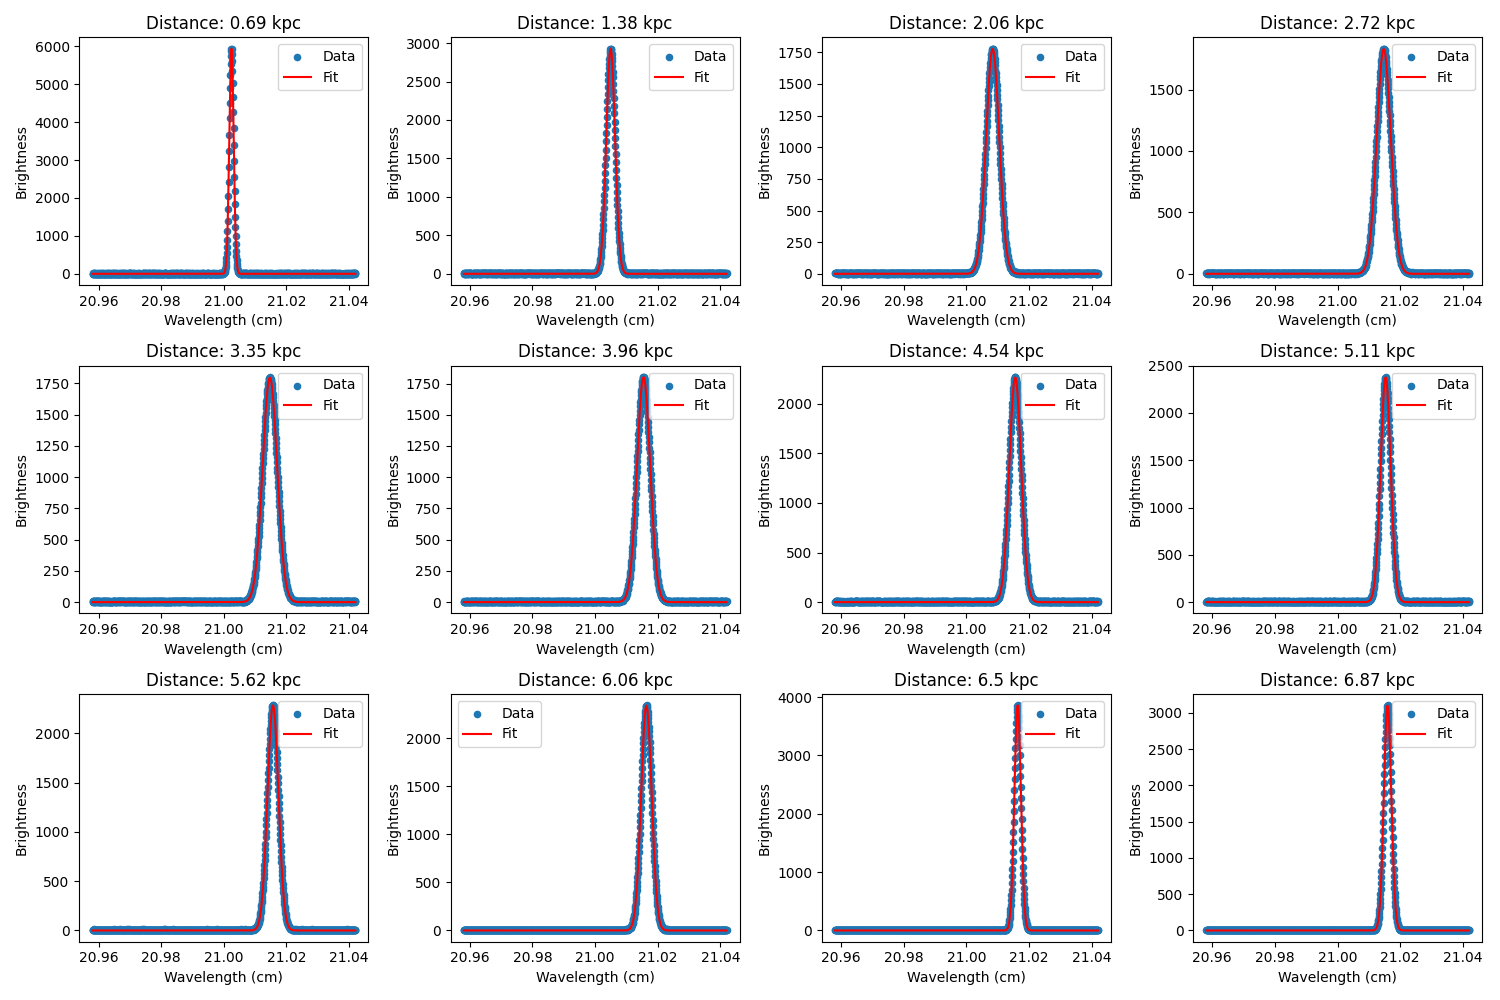
\includegraphics[width=\textwidth]{Images/12_files.png}
	\caption{Plots for each distance}
	\label{fig:12_files}
\end{figure}

Using the data obtained from the Gaussian fits, we can plot the velocities as a function of distance from the centre of the galaxy. 

\begin{figure}[H]
	\centering
	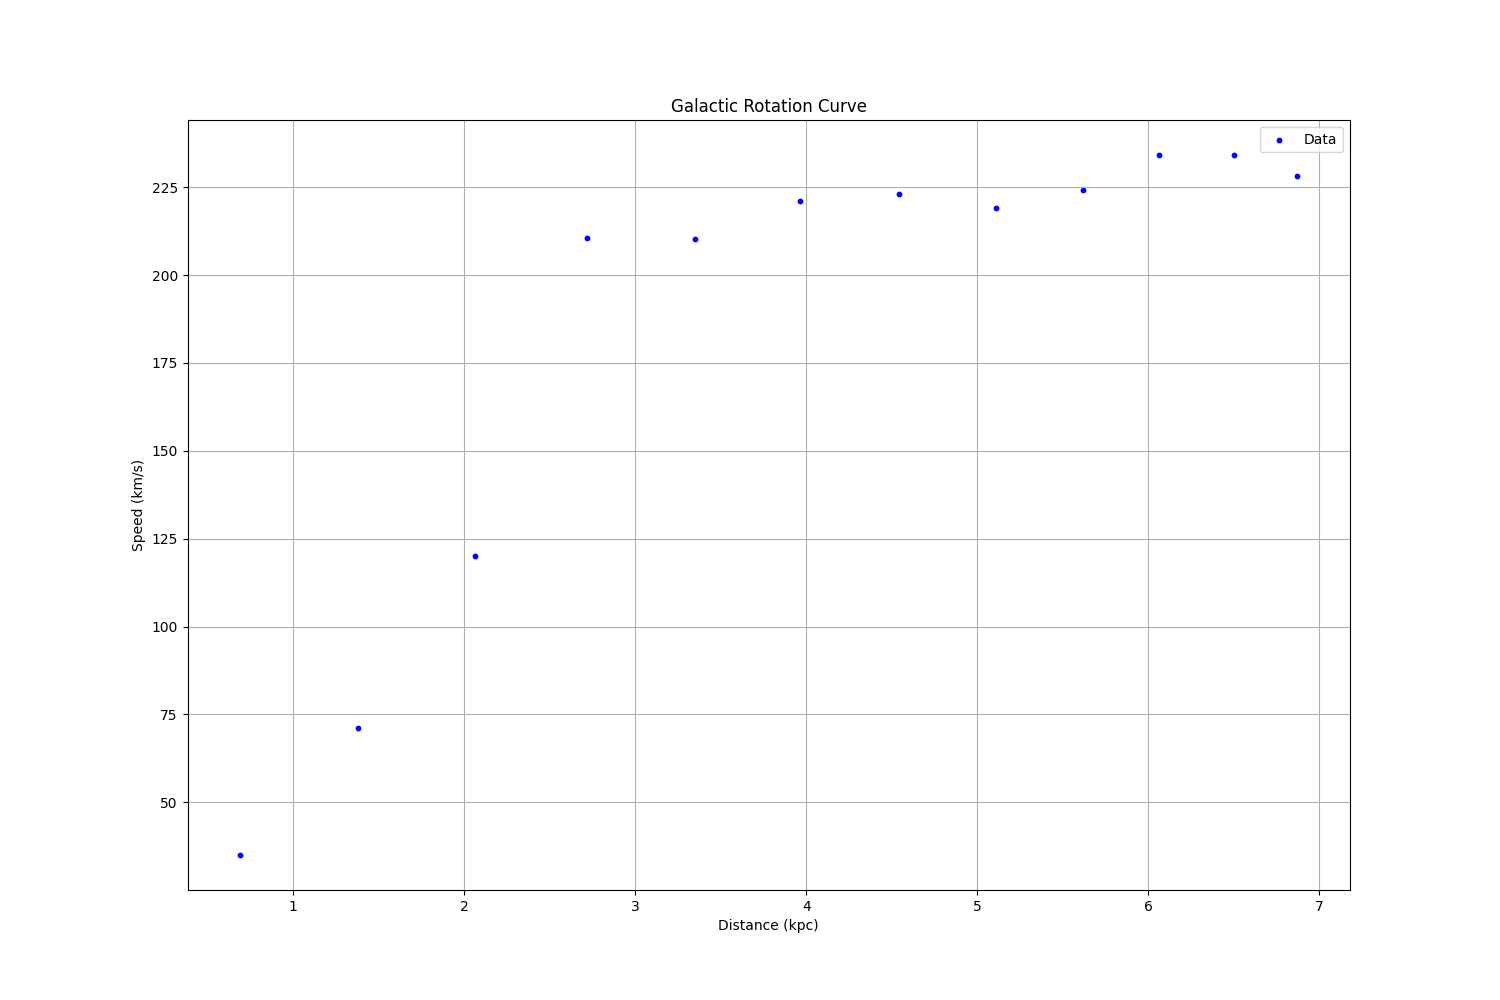
\includegraphics[width=\textwidth]{Images/galaxy_rotation_curve.png}
	\caption{Galaxy Rotation Curve}
	\label{fig:galaxy_rotation_curve}
\end{figure}